\documentclass[a4paper, twoside, 11pt]{article}
\input{../preamble}
\usepackage{graphicx}
%\graphicspath{{figures}}


%\usepackage{multicol}
%\setlength{\columnsep}{1cm}

\titleformat{\section}{\centering\normalfont\huge\bfseries}{\thesection}{1em}{}
\titleformat{\subsection}{\centering\normalfont\Large\bfseries}{\thesubsection}{1em}{}
%\titleformat{\subsection}{\centering\normalfont\large\bfseries\MakeUppercase}{\thesubsection}{1em}{}

\fancypagestyle{fheaders}{
    \fancyhead{}
    \fancyfoot{}
    \fancyhead[RE]{Configure, evaluate and select a hardware platform - Part 2}
    \fancyhead[LO]{Configure, evaluate and select a hardware platform - Part 2}
    \fancyfoot[C]{\thepage}
}

\pagestyle{fheaders}

\begin{document}

\begin{titlepage}
\topskip0pt
\vspace*{\fill}
\begin{center}
\thispagestyle{noheaders}
\Huge\textbf{Configure, evaluate and select a hardware platform - Part 2}
\vskip0.5cm
\large Computer Hardware lab report 
\vskip0.1cm Group 1191 - 1st October 2020 
\vskip1cm
%\hr
%\vskip1cm
\large Álvaro Cortizas Tarrón,\ Javier García Regidor
\vskip0.5cm
\end{center}
\vspace*{\fill}
\end{titlepage}

\thispagestyle{noheaders}
\topskip0pt
\vspace*{\fill}
\tableofcontents
\vspace*{\fill}
\newpage

%\thispagestyle{noheaders}

\section{Introduction}
\hspace{\parindent} In this report, we are  

%, specialy at the time of buying one, as well as the differences in the CPUs from the main manufacturers.


%Over time, processors have evolved from a single processing chip to larger chips containing multiple processors called \textit{cores}, increasing the computational power. In the following sections of this report will be discussed some terminology and characteristics of microprocessors that are worth consider knowing, specialy at the time of buying one, as well as the differences in the CPUs from the main manufacturers.
%\vskip1cm
%\begin{multicols}{2}
%\end{multicols}

\section{Build specifications}

%\begin{multicols}{2}
\subsection{Microprocessor}
\hspace{\parindent} The microprocessor is a crucial component when running software such as AutoCAD and videogames. 

\hspace{\parindent} Although the term \textit{microprocessor} is most commonly used to refer to the CPU, it can also refer to another kind  of microprocessors such as \textit{co-processors} or \textit{GPUs (Graphics Processing Units)}.



\subsection{Motherboard}


\subsection{RAM memory}



\subsection{Graphics card (GPU)}


\subsection{Storage}

\subsection{Cooling}


\subsection{Power supply}


\subsection{Chasis}


\subsection{Peripherals}



\hide{
\subsection{Types of microprocessors}
\hspace{\parindent} Microprocessors can be classified as follows:
\begin{itemize}
    \hide{
    \item\textbf{RISK.} These microprocessors execute simple instructions such as loading data from memory, resulting in a higher performance when the architecture of the microprocessor can execute those instructions using fewer cycles.
    \item\textbf{CISC.} CISC is a type of microprocessors that allows to run more complex instructions. The design is such that single instructions can execute several low-level operations (like loading or storing data on memory). Also, they are capable of executing multi-step operations and addressing modes within single instructions.
    }
    \item\textbf{Scalar CPU.} A scalar CPU is the one which performs computations on a single number or a set of data at a time.
    \item\textbf{Array CPU.} It is a type of microprocessor that allows a single instruction to operate at the same time on multiple sets of data.
    \item\textbf{Parallel processors.} These uses independent processors to work on the same program. The process is split into different tasks, each of which can be processed by any of the processors. 
\end{itemize}
\subsection{Terminology and specifications}
The following is a list of the main terminology and specifications related to microprocessors:
\begin{itemize}
    \item\textbf{Architecture.} The logic design of microprocessors is called the \textit{architecture} of the processor. In order to perform operations on input data, each microprocessor has a set of instructions designed internally, the ISA, which stands for Instruction Set Architecture, from which we can define the architecture. Talking about the ISA, we can distinguise between RISC (Reduced Instruction Set Computer), which execute simple instructions, and CISC (Complex Instruction Set Computer) microprocessors, which can run more complex instructions. 
        
        The most common microprocessor architecture today is x86, which is implemented in both 32-bit and 64-bits (x86-64) microprocessors. Most of the 64-bit microprocessors today are x86-64 CISC, but there are still 64-bit RISC microprocessors that uses other architectures, such as ARM.

    \item\textbf{Cores.} Nowadays, computers have multicore processors, meaning that each of them is comprised of two or more CPUs, called cores. This technology leads to an increase on the performance of software written to use more than one core at the same time, as individual cores can execute multiple instructions in parallel. 

    \item\textbf{Threads.} Most processors can use a process called \textit{simultaneous multithreading} to split a core into virtual, or logical cores, called \textit{threads}. This technology is pretty useful when performing multiple tasks at the same time (as each thread can act as an individual core performing different tasks) or when running demanding software, for example, video editing and animation software.
    \item\textbf{Socket.} A CPU socket is a connection between the microprocessor and the motherboard composed of a series of pins. The main benefit of a socket is that the microprocessor is not directly soldered and can be easily placed and replaced without much effort. It is also worth mentioning that not every CPU work with any CPU socket, so we need to make sure the motherboard has the right CPU socket before getting a microprocessor. Sockets are usually classified into Pin Grid Array (PGA) and Land Grid Array (LGA) depending on the placement of the pins. Common CPU sockets are the AM4 from AMD's Ryzen processors and the LGA 1151 from Intel's 8th and 9th generation Core processors.
    \begin{center}
        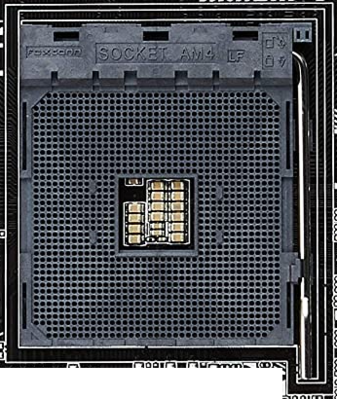
\includegraphics[width=0.3\textwidth]{./figures/am4-socket.png}
        \captionof{figure}{AM4 socket from an AMD microprocessor.}
    \end{center}

\item\textbf{Cache memory.} It's a volatile computer memory from which the CPU can retrieve data frequenty used by computer programs in an easy and efficient way. It is sometimes called \textit{CPU memory} of its physical proximity to it, as we can find it directly integrated into the CPU chip. For this reason it is considered the fastest memory in a computer. However, they have a very limited size. 

    Depending on its read/write speed it is classified into L1 (Level 1 Cache), L2 (Level 2 Cache), L3 (Level 3 Cache) from faster to slower.    
    \begin{center}
        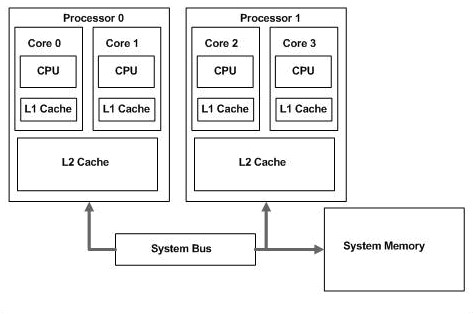
\includegraphics[width=0.7\textwidth]{./figures/memory-diagram.jpeg}
        \captionof{figure}{Cache memory integrated in a microprocessor chip.}
    \end{center}

\newpage
\item\textbf{Clock frequency.} The clock frequency is a way to measure processor performance. It refers to the speed of the clock inside the CPU and, in general, a higher clock frequency implies a faster CPU. The clock frequency, also known as clock speed, measures the number of cycles of the CPU executes per second, usually in gigahertz (GHz). In a few words, a \textit{cycle} is kind of the number of completed instructions in a tiny interval of time. 

    For instance, a CPU with a clock frequency of 4.2 GHz would be able to execute 4.2 billion cycles per second. It should be taken into account when looking for a new microprocessor that a higher clock frequency implies more power consumption. 

    \item\textbf{Overlock.} As the name suggests, overlocking a CPU means increasing its clock frequency in order to get a higher performance, but at the cost of a higher power consumption. Furthermore, if it is not done properly it can cause damage to the microprocessor by overheating.

    \item\textbf{Power consumption.} The power consumption of a microprocessor is the necessary electrical power for the CPU to operate properly, usually measured in watts (W). It may seem obvious that a more powerful CPU will have a higher power consumption and viceversa.

    \hide{
    \item\textbf{Data width.} The ALU (Arithmetic Logic Unit) is a digital circuit integrated in the CPU primarly in charge of arithmetic operations. Data width refers to the width of the ALU. For instance, a 32-bit ALU can operate with 32-bit numbers. A wider ALU implies operating with larger numbers using lower amount of instructions.
    \item\textbf{MIPS.} MIPS stands for \textit{millions of instructions per second} and is a rough measure of the performance of a CPU. Modern CPUs can do so many different things that MIPS ratings lose a lot of their meaning, but you can get a general sense of the relative power of the CPUs. In general, there is a relationship between clock speed and MIPS. The maximum clock speed is a function of the manufacturing process and delays within the chip. 
    }
\end{itemize}

\subsection{Main processor manufacturers in the market}
\hspace{\parindent} Nowadays, there are two main microprocessors manufacturers: Intel and AMD. According to our necessities a CPU from one manufacturer will benefit us more than one from another manufacturer. In this section, we will be discussing the different characteristics of both Intel's and AMD's microprocessors.

To begin with, Intel's CPUs as a great single-core power, suitable for demanding tasks, specially gaming. They also have a higher energetic efficiency than AMD's, which helps reducing the overall power consumption. However, Intel's microprocessors tend to have also a higher price, and in some cases last generation CPUs are not affordable by many people.

Although AMD processors has a higher number of cores, which is a great feature in case of carrying out multiple tasks at the same time, are less powerful in terms of single-core power. For this reason, many tend to buy mid-range Intel's processors than AMD's.

In the following table are summarized the main characteristics of Intel and AMD microprocessors.
\bgroup
\def\arraystretch{1.2}
\begin{table}[h!]
\centering
\begin{tabular}{|c|c|}\hline
    \textbf{Intel microprocessors} & \textbf{AMD microprocessors} \\
    \hline
    Higher single-core power & Lower single-core power \\
    \hline
    Lower number of cores and threads & Higher number of cores and threads \\
    \hline
    More energy efficient & Not so energy efficient \\
    \hline
    Pricier & Cheaper \\
    \hline
\end{tabular}
\caption{Comparison between Intel and AMD microprocessors.}
\end{table}
\egroup

\subsection{What is the SKU of a processor?}
\hspace{\parindent} SKU, which stands for \textit{Stock Keeping Unit} is a number or string of alphanumeric characters that are used to indentify a certain product. Let's analyse the SKU of Intel microprocessors, which is divided into five parts.

\begin{center}
    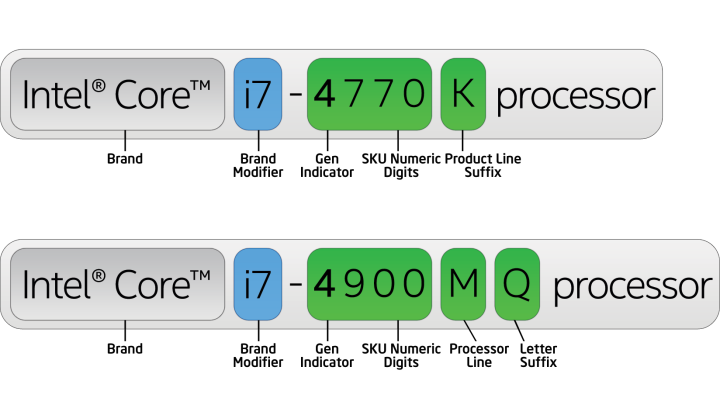
\includegraphics[width=0.6\textwidth]{./figures/intel-sku.png}
    \captionof{figure}{SKU example from an Intel microprocessor.}
\end{center}

\begin{itemize}
    \item\textbf{Brand.} This is the name of the processor and the product line to which it belongs. Nowadays, the most common are Intel Core, Intel Pentium and AMD Ryzen in AMD's case.

    \item\textbf{Brand modifier.} Intel Core processors includes the brand modifiers i3, i5, i7 and i9 to refer to low, mid and high range. Higher brand modifier numbers offer an overall greater performance and, in some cases, additional features, as well as a higher power consumption.

    \item\textbf{Generation indicator.} The first digit of the following four-digit processor number is called the \textit{generation indicator} and, as its name suggest, represents the generation to which the processor belongs (except 10th generation processors).

    \item\textbf{SKU numeric digits.} For the vast majority of Intel processors, the final three digits of the product number are the reference number for that specific processor. 

    \item\textbf{Product line suffix.} The product line suffix indicates some key characteristic of the processor. For instance, SKU suffixies with a $H$ means that the processor has a higher performance and is optimized for laptops. Other Intel processors suffixies are \textit{G1-G7} (graphics level), \textit{E} (embedded), \textit{F} (requires discrete graphics), \textit{G} (includes discrete graphics), \textit{K} (unlocked), \textit{S} (special edition), \textit{T} (power-optimized lifestyle), \textit{U} (mobile power efficient), \textit{Y} (mobile extremely low power), \textit{H} (high performance optimized for mobile), \textit{HK} (high performance optimized for mobile, unlocked), \textit{HQ} (high performance optimized for mobile, quad core).
\end{itemize}
%\end{multicols}
}

\section{Conclusions}
\hspace{\parindent} Microprocessors are very complex components that, as many other components of a computer, require some knowledge and previous research in order to distinguise their different types and choose the one that is more suitable for our system, taking into account both hardware and necessities.

\addcontentsline{toc}{section}{References}
\begin{thebibliography}{11}
    \bibitem{wiki-cpu}
    Wikipedia. \textit{Central Processing Unit}. \\\texttt{en.wikipedia.org/wiki/Central\textunderscore processing\textunderscore unit}

    \bibitem{wiki-processor}
    Wikipedia. \textit{Processor (computing)}. \\\texttt{en.wikipedia.org/wiki/Processor\textunderscore(computing)}

    \bibitem{hsw-microprocessor}
    How stuff works. \textit{Microprocessor}. \\\texttt{computer.howstuffworks.com/microprocessor.htm}

    \bibitem{types-of-processors2}
    Java T Point. \textit{Evolution of Microprocessors}. \\\texttt{javatpoint.com/types-of-microprocessors}

    \bibitem{types-of-processors}
    Wikibooks. \textit{Unit 1.1.2 Types of Processor}. \\\texttt{en.wikibooks.org/wiki/A-level\textunderscore Computing/OCR/Unit\textunderscore 1.1.2\textunderscore Types\textunderscore of\textunderscore Processor}

    \bibitem{pccomponentes}
    PC Componentes. \textit{Procesador CPU ¿Qué es? Características y tipos}. \\\texttt{pccomponentes.com/procesador-cpu-que-es-caracteristicas-tipos}

    \bibitem{cpu-socket}
    Tom's Hardware. \textit{What is a CPU socket? A basic definition}. \\\texttt{tomshardware.com/reviews/cpu-socket-definition,5758.html}

    \bibitem{cache-memory}
    Tech Target. \textit{Cache memory}. \\\texttt{searchstorage.techtarget.com/definition/cache-memory}

    \bibitem{cache-memory2}
    Technopedia. \textit{Cache Memory}. \\\texttt{technopedia.com/definition/6307/cache-memory}

    \bibitem{intel-sku}
    Intel. \textit{Processor numbers}. \\\texttt{intel.com/content/www/us/en/processors/processor-numbers.html}

    \bibitem{sku-report}
Studocu. \textit{Práctica de laboratorio sobre procesadores y lenguaje ensamblador}. \\\texttt{studocu.com/ec/document/universidad-catolica-de-cuenca/arquitectura-de-} \\\texttt{hardware/informe/practica-del-laboratorio-sobre-procesadores-y-lenguaje-} \\\texttt{ensamblador/5972562/view}
\end{thebibliography} 
\end{document}
